\chapter{API Reference}
\label{chapter-API}

This appendix provides an API reference for the software that has been
developed as part of this thesis.

\section{Graph Node Classes}

Objects of the \texttt{ezcWorkflowNode} classes represent the nodes of a
workflow.

\subsection{ezcWorkflowNode}

\texttt{ezcWorkflowNode} (see Figure \ref{classezcWorkflowNode}) is the
abstract base class for all graph node classes.

\begin{figure}[p!]
\begin{center}
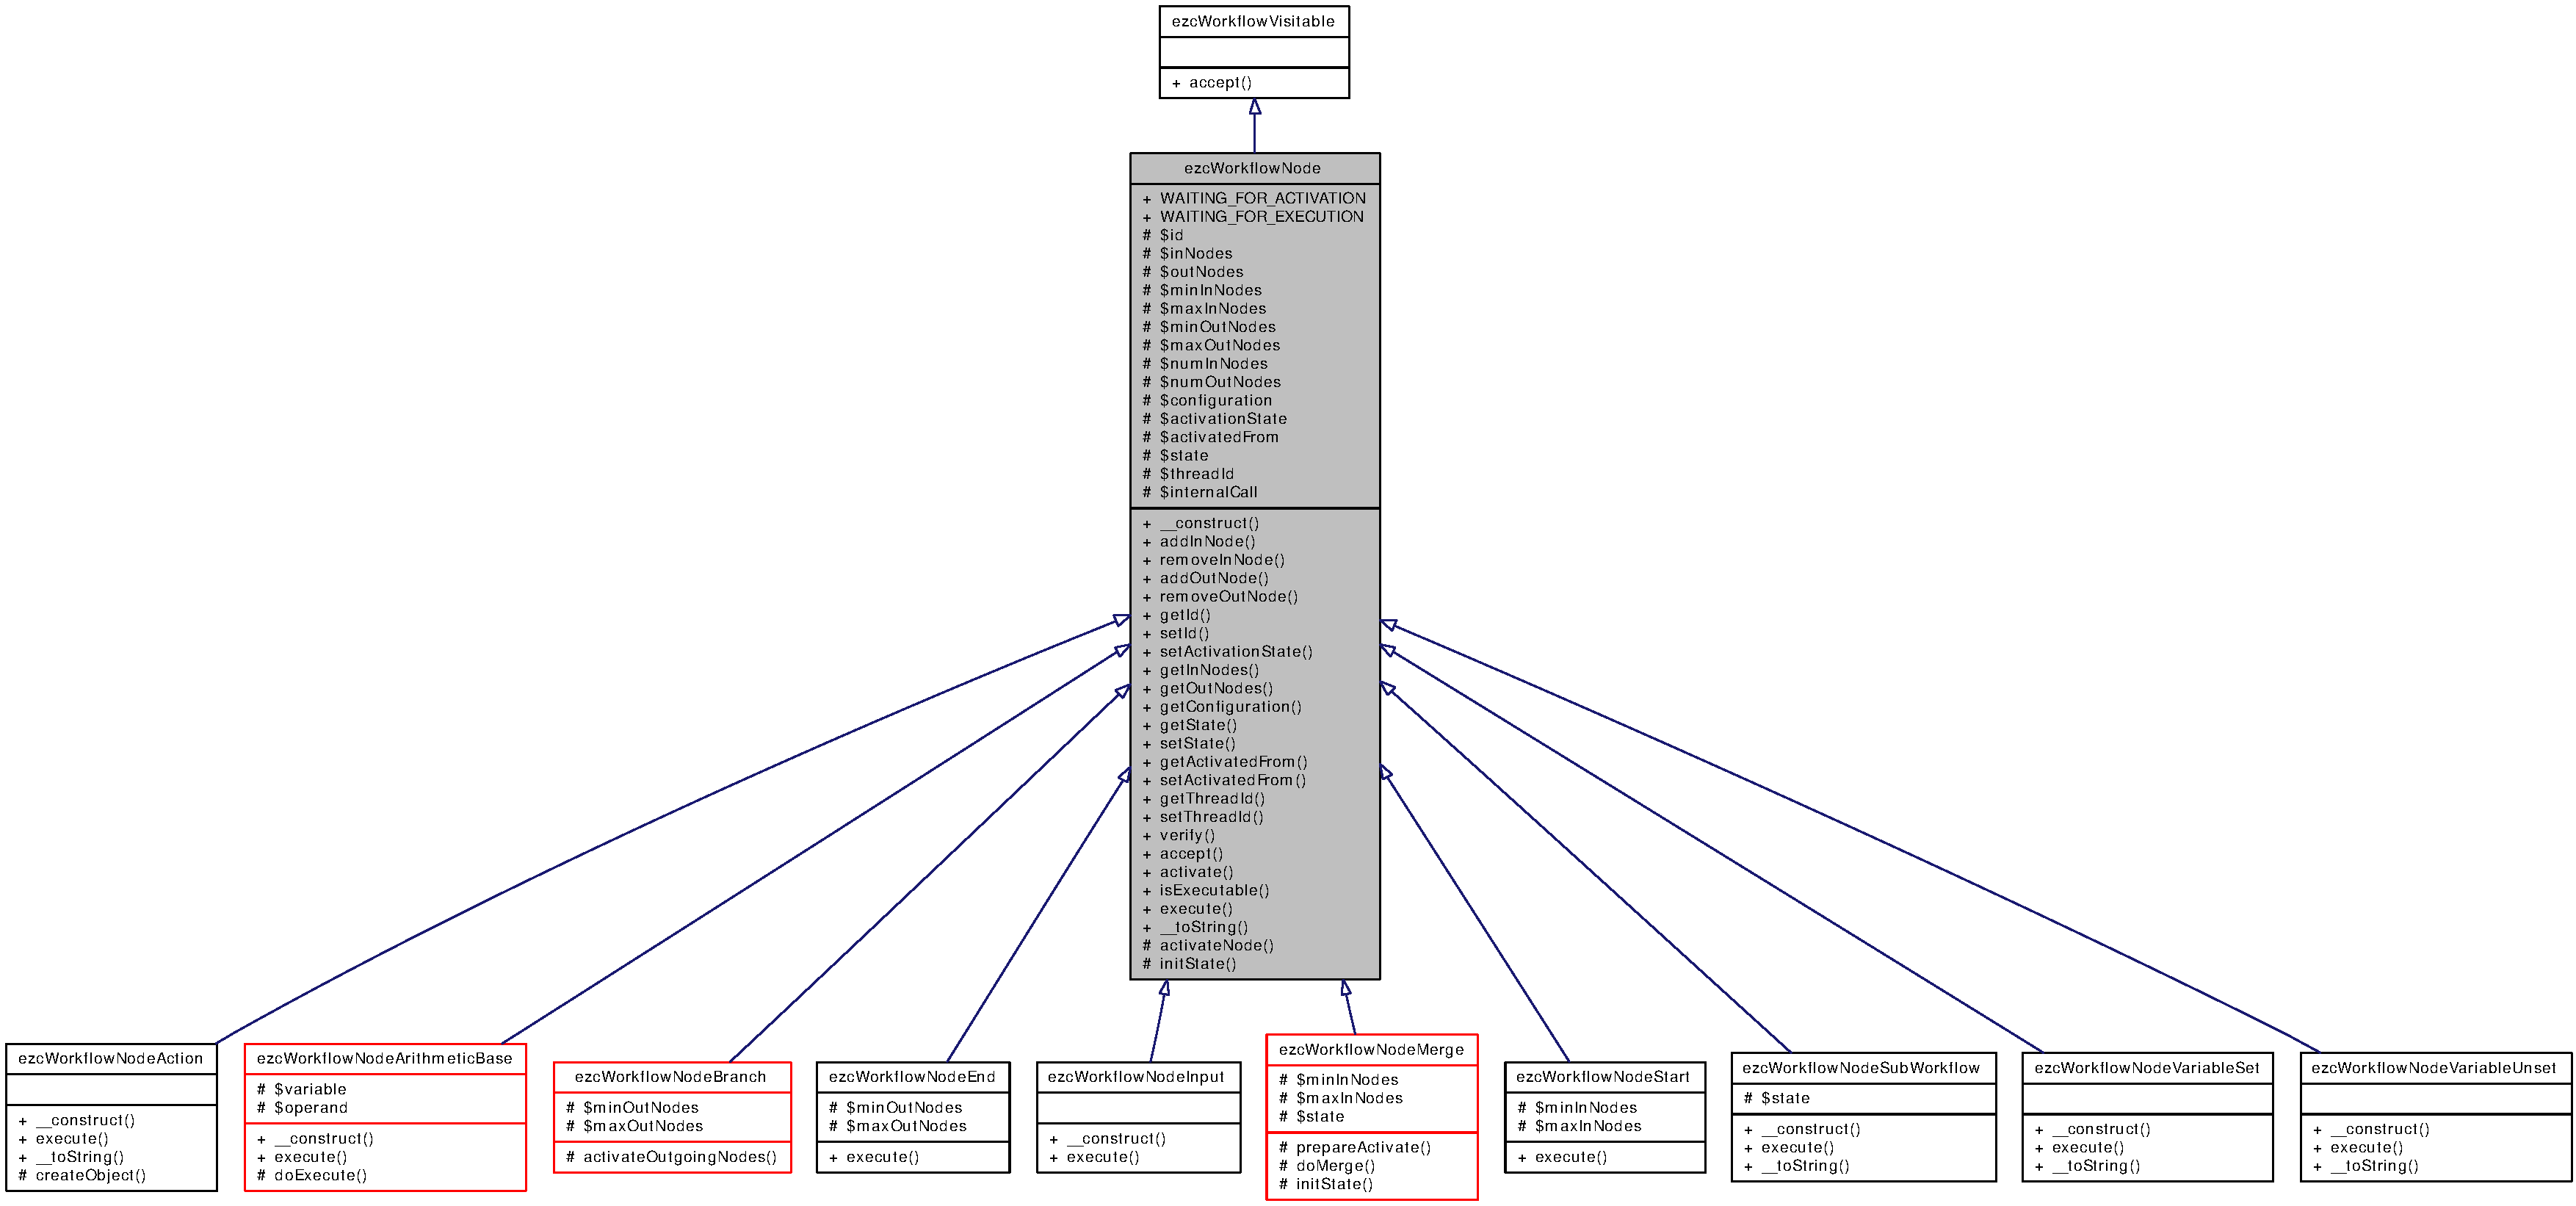
\includegraphics[angle=90,width=10cm]{figures/WorkflowNode}\\[5mm]
\end{center}
\caption{The \texttt{ezcWorkflowNode} class and its subclasses}
\label{classezcWorkflowNode}
\end{figure}

\subsection{Start and End Nodes}

\subsubsection{ezcWorkflowNodeStart}

\emph{Incoming Nodes: 0}\\
\emph{Outgoing Nodes: 1}\\

An object of the \texttt{ezcWorkflowNodeStart} class (see
Figure~\ref{classezcWorkflowNode}) represents the one and only start node of a
workflow. The execution of the workflow starts here.

Creating an object of the \texttt{ezcWorkflow} automatically creates the
start node for this new workflow.

\begin{lstlisting}[language=PHP]
$workflow = new ezcWorkflow( 'Name' );
$workflow->startNode; // This property holds the ezcWorkflowNodeStart object.
\end{lstlisting}

\subsubsection{ezcWorkflowNodeEnd}

\emph{Incoming Nodes: 1}\\
\emph{Outgoing Nodes: 0}\\

An object of the \texttt{ezcWorkflowNodeEnd} class (see
Figure~\ref{classezcWorkflowNode}) represents an end node of a workflow. A
workflow must have at least one end node. The execution of the workflow ends
when an end node is reached.

Creating an object of the \texttt{ezcWorkflow} automatically creates a default
end node for this new workflow.

\begin{lstlisting}[language=PHP]
$workflow = new ezcWorkflow( 'Name' );
$workflow->endNode; // This property holds an ezcWorkflowNodeEnd object.
\end{lstlisting}

\subsubsection{ezcWorkflowNodeCancel}

\emph{Incoming Nodes: 1}\\
\emph{Outgoing Nodes: 0..1}\\

The \texttt{ezcWorkflowNodeCancel} class implements the
\emph{Cancel Case} workflow pattern.

\begin{lstlisting}[language=PHP]
$workflow = new ezcWorkflow( 'Name' );
$workflow->endNode = new ezcWorkflowNodeCancel;
\end{lstlisting}

As soon as a node of the \texttt{ezcWorkflowNodeCancel} type is activated, the
complete workflow instance is removed. This includes currently executing nodes,
those which may execute at some future time and all parent and sub-workflows.
The workflow instance is recorded as having completed unsuccessfully.

\subsubsection{ezcWorkflowNodeFinally}

\emph{Incoming Nodes: 0}\\
\emph{Outgoing Nodes: 1}\\

An object of the \texttt{ezcWorkflowNodeFinally} class (see
Figure~\ref{classezcWorkflowNode}) represents the start node of a sequence of
final activities that is executed when a workflow execution is cancelled.

Creating an object of the \texttt{ezcWorkflow} class automatically creates the
finally node for this new workflow.

\begin{lstlisting}[language=PHP]
$workflow = new ezcWorkflow( 'Name' );
$workflow->endNode = new ezcWorkflowNodeCancel;
$workflow->finallyNode->addOutNode( /* ... */ );
\end{lstlisting}

\subsection{ezcWorkflowNodeAction}

\emph{Incoming Nodes: 1}\\
\emph{Outgoing Nodes: 1}\\

An object of the \texttt{ezcWorkflowNodeAction} class (see
Figure~\ref{classezcWorkflowNode}) represents an activity node. When the node
is reached, the business logic that is implemented by the associated
\emph{service object} is executed.

\begin{lstlisting}[language=PHP]
class MyAction implements ezcWorkflowServiceObject
{
    public function execute( ezcWorkflowExecution $execution )
    {
        // ...
    }

    public function __toString()
    {
        // ...
    }
}

$action = new ezcWorkflowNodeAction( 'MyAction' );
\end{lstlisting}

\subsection{ezcWorkflowNodeSubWorkflow}

\emph{Incoming Nodes: 1}\\
\emph{Outgoing Nodes: 1}\\

An object of the \texttt{ezcWorkflowNodeSubWorkflow} class (see
Figure~\ref{classezcWorkflowNode}) represents a sub-workflow. When the node
is reached, the specified sub-workflow is started. The workflow is suspended
until the sub-workflow has finished executing.

\begin{lstlisting}[language=PHP]
$subWorkflow = new ezcWorkflow( 'Sub-Workflow Name' );
// ...

$subWorkflow = new ezcWorkflowNodeSubWorkflow( 'Sub-Workflow Name' );
\end{lstlisting}

Workflow variables can be passed from the parent workflow to the
child worflow and vice versa. The example below creates a sub-workflow
node that passes the parent execution's variable \texttt{x} to the variable
\texttt{y} in the child execution when the sub-workflow is started. When it
ends, the child execution's \texttt{y} variable is passed to the parent
execution as \texttt{z}.

\begin{lstlisting}[language=PHP]
$subWorkflow = new ezcWorkflow( 'Sub-Workflow Name' );
// ...

$subWorkflow = new ezcWorkflowNodeSubWorkflow(
  array(
    'workflow'  => 'IncrementVariable',
    'variables' => array(
      'in' => array(
        'x' => 'y'
      ),
      'out' => array(
        'y' => 'z'
      )
    )
  )
);
\end{lstlisting}

\subsection{Workflow Variables}

\subsubsection{ezcWorkflowNodeInput}

\emph{Incoming Nodes: 1}\\
\emph{Outgoing Nodes: 1}\\

An object of the \texttt{ezcWorkflowNodeInput} class (see
Figure~\ref{classezcWorkflowNode}) represents an input node. When the node is
reached, the workflow engine will suspend the workflow execution if the
specified input data is not available (first activation). While the workflow
is suspended, the application that embeds the workflow engine may supply the
input data and resume the workflow execution (second activation of the input
node). Input data is stored in a workflow variable.

\subsubsection{ezcWorkflowNodeVariableSet}

\emph{Incoming Nodes: 1}\\
\emph{Outgoing Nodes: 1}\\

An object of the \texttt{ezcWorkflowNodeVariableSet} class sets a specified
workflow variable to a given value.

\begin{lstlisting}[language=PHP]
$set = new ezcWorkflowNodeVariableSet(
  array( 'variable name' => $value )
);
\end{lstlisting}

\subsubsection{ezcWorkflowNodeVariableUnset}

\emph{Incoming Nodes: 1}\\
\emph{Outgoing Nodes: 1}\\

An object of the \texttt{ezcWorkflowNodeVariableUnset} class unsets a
specified workflow variable.

\begin{lstlisting}[language=PHP]
$unset = new ezcWorkflowNodeVariableUnset( 'variable name' );
\end{lstlisting}

\begin{figure}[hbt]
\begin{center}
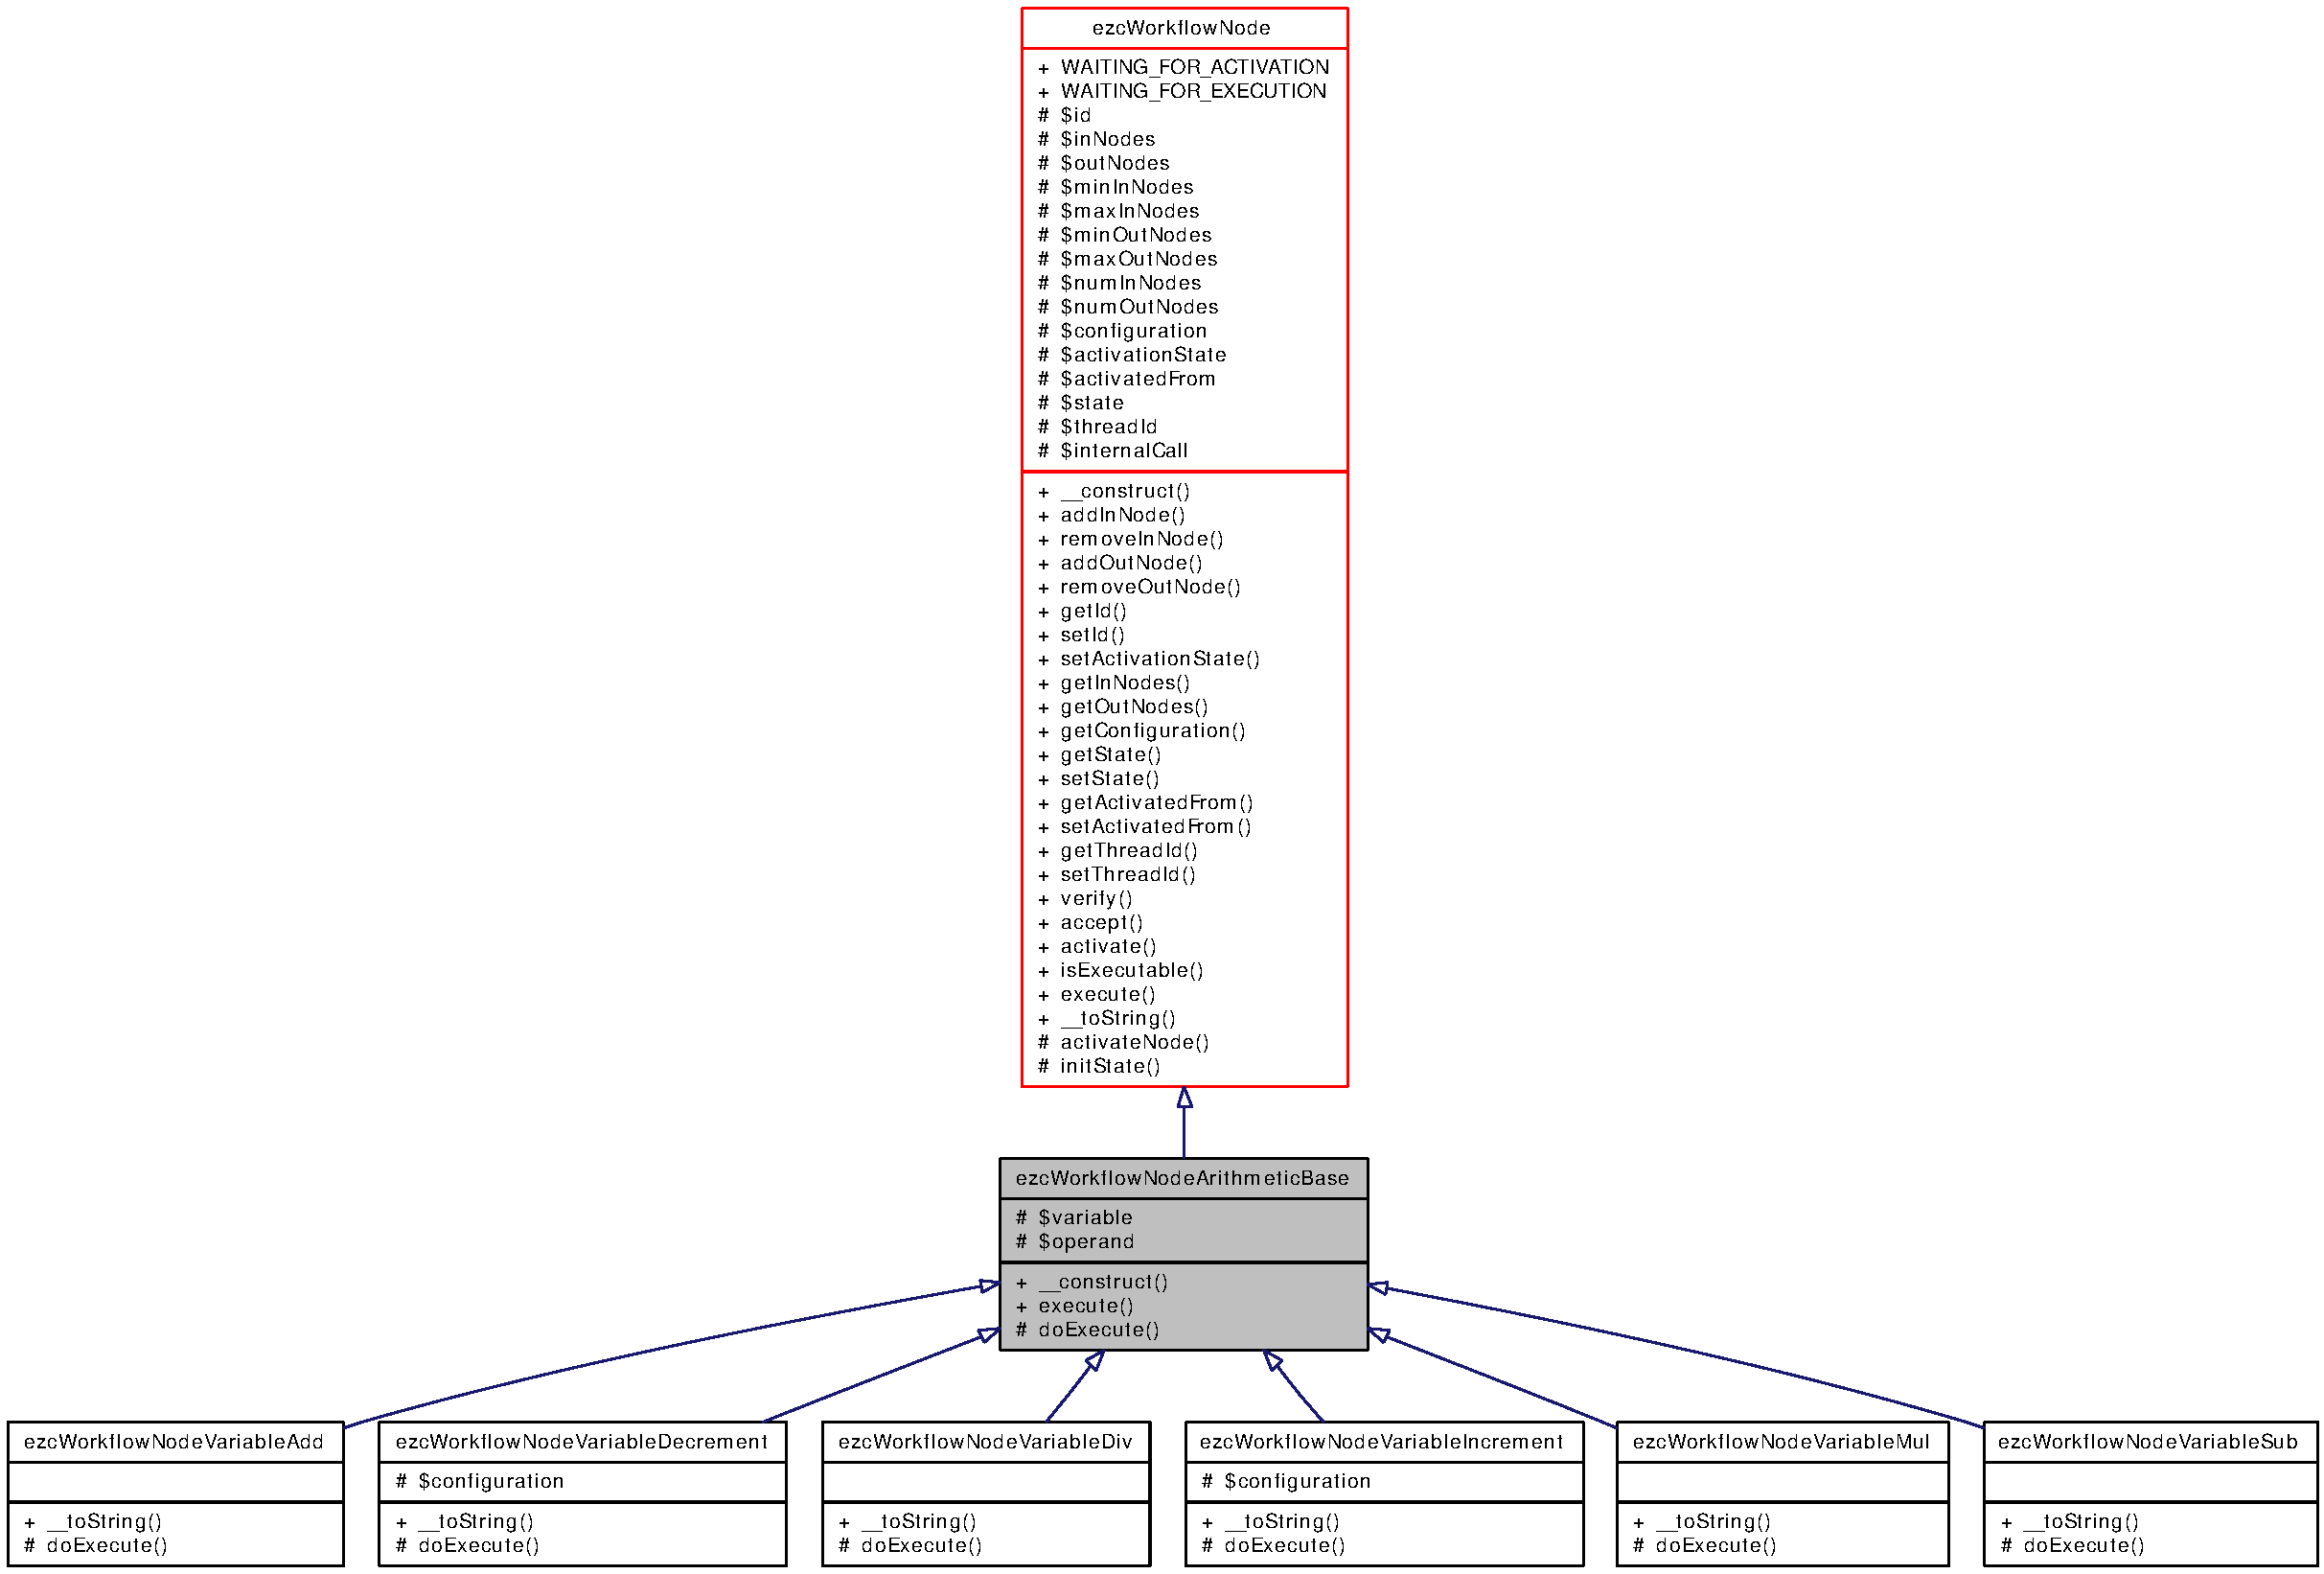
\includegraphics[width=16cm]{figures/WorkflowNodeArithmeticBase}\\[5mm]
\end{center}
\caption{The \texttt{ezcWorkflowNodeArithmeticBase} class and its subclasses}
\label{classezcWorkflowNodeArithmeticBase}
\end{figure}

\subsubsection{ezcWorkflowNodeVariableAdd}

\emph{Incoming Nodes: 1}\\
\emph{Outgoing Nodes: 1}\\

An object of the \texttt{ezcWorkflowNodeVariableAdd} class adds a given value,
either a constant or the value of another workflow variable, to a specified
workflow variable.

\begin{lstlisting}[language=PHP]
$add = new ezcWorkflowNodeVariableAdd(
  array( 'name' => 'variable name', 'value' => $value )
);
\end{lstlisting}

When \texttt{\$value} is a string, the value of the variable identified by
that string is used.

\subsubsection{ezcWorkflowNodeVariableSub}

\emph{Incoming Nodes: 1}\\
\emph{Outgoing Nodes: 1}\\

An object of the \texttt{ezcWorkflowNodeVariableSub} class subtracts a given
value, either a constant or the value of another workflow variable, from a
specified workflow variable.

\begin{lstlisting}[language=PHP]
$sub = new ezcWorkflowNodeVariableSub(
  array( 'name' => 'variable name', 'value' => $value )
);
\end{lstlisting}

When \texttt{\$value} is a string, the value of the variable identified by
that string is used.

\subsubsection{ezcWorkflowNodeVariableMul}

\emph{Incoming Nodes: 1}\\
\emph{Outgoing Nodes: 1}\\

An object of the \texttt{ezcWorkflowNodeVariableMul} class multiplies a specified
workflow variable with a given value, either a constant or the value of another
workflow variable.

\begin{lstlisting}[language=PHP]
$mul = new ezcWorkflowNodeVariableMul(
  array( 'name' => 'variable name', 'value' => $value )
);
\end{lstlisting}

When \texttt{\$value} is a string, the value of the variable identified by
that string is used.

\subsubsection{ezcWorkflowNodeVariableDiv}

\emph{Incoming Nodes: 1}\\
\emph{Outgoing Nodes: 1}\\

An object of the \texttt{ezcWorkflowNodeVariableDiv} class divides a specified
workflow variable by a given value, either a constant or the value of another
workflow variable.

\begin{lstlisting}[language=PHP]
$div = new ezcWorkflowNodeVariableDiv(
  array( 'name' => 'variable name', 'value' => $value )
);
\end{lstlisting}

When \texttt{\$value} is a string, the value of the variable identified by
that string is used.

\subsubsection{ezcWorkflowNodeVariableIncrement}

\emph{Incoming Nodes: 1}\\
\emph{Outgoing Nodes: 1}\\

An object of the \texttt{ezcWorkflowNodeVariableIncrement} class increments
the value of a specified workflow variable.

\begin{lstlisting}[language=PHP]
$inc = new ezcWorkflowNodeVariableIncrement( 'variable name' );
\end{lstlisting}

\subsubsection{ezcWorkflowNodeVariableDecrement}

\emph{Incoming Nodes: 1}\\
\emph{Outgoing Nodes: 1}\\

An object of the \texttt{ezcWorkflowNodeVariableDecrement} class decrements
the value of a specified workflow variable.

\begin{lstlisting}[language=PHP]
$dec = new ezcWorkflowNodeVariableDecrement( 'variable name' );
\end{lstlisting}

\subsection{Workflow Patterns}

\subsubsection{ezcWorkflowNodeParallelSplit}

\emph{Incoming Nodes: 1}\\
\emph{Outgoing Nodes: 2 \dots *}\\

The \texttt{ezcWorkflowNodeParallelSplit} class implements the
\emph{Parallel Split} workflow pattern.

\begin{figure}[hbt]
\begin{center}
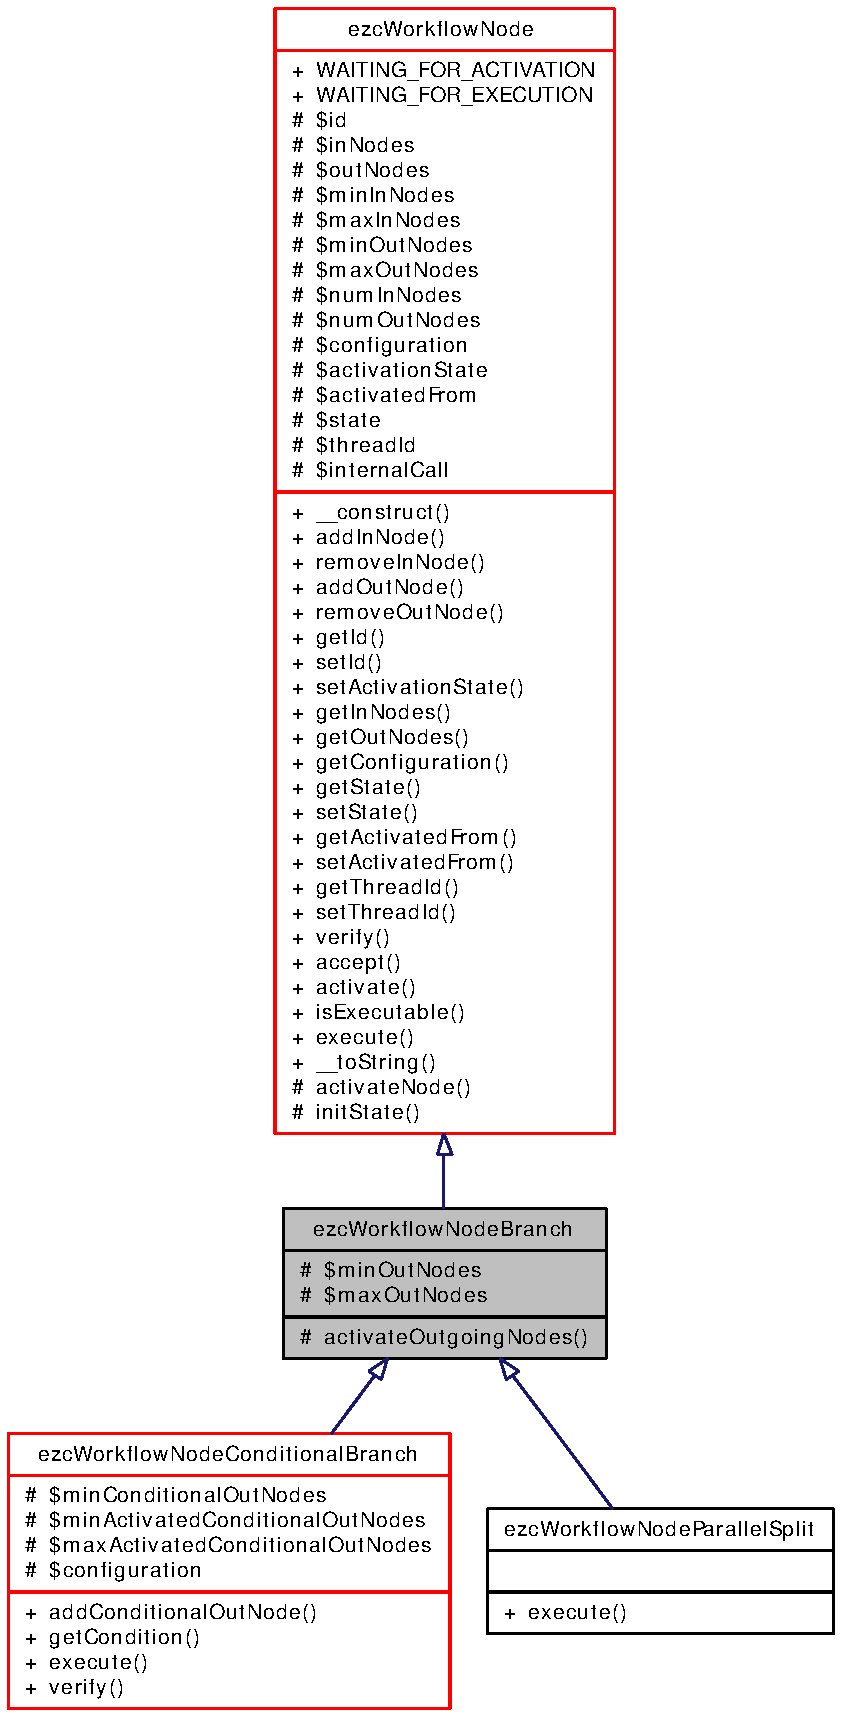
\includegraphics[width=10cm]{figures/WorkflowNodeBranch}\\[5mm]
\end{center}
\caption{The \texttt{ezcWorkflowNodeBranch} class and its subclasses}
\label{classezcWorkflowNodeBranch}
\end{figure}

\subsubsection{ezcWorkflowNodeSynchronization}

\emph{Incoming Nodes: 2 \dots *}\\
\emph{Outgoing Nodes: 1}\\

The \texttt{ezcWorkflowNodeSynchronization} class implements the
\emph{Synchronization} workflow pattern.

\begin{figure}[hbt]
\begin{center}
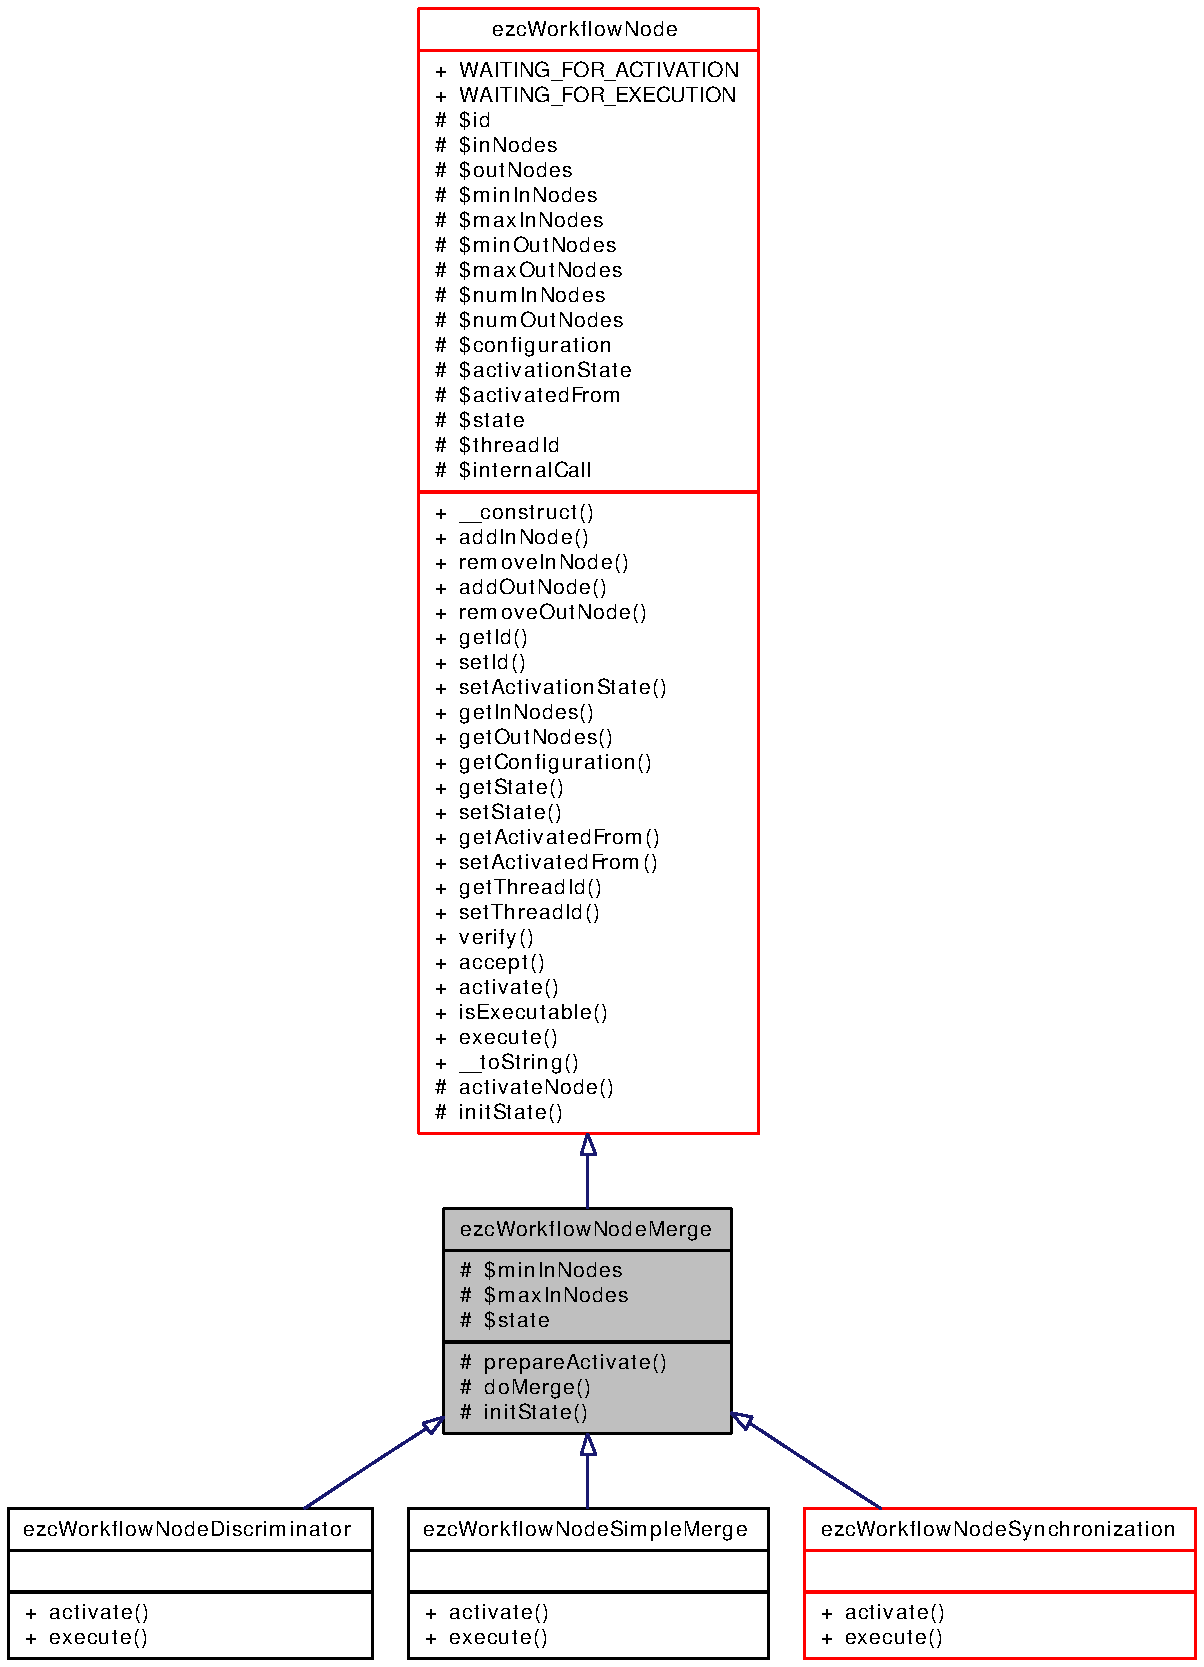
\includegraphics[width=10cm]{figures/WorkflowNodeMerge}\\[5mm]
\end{center}
\caption{The \texttt{ezcWorkflowNodeMerge} class and its subclasses}
\label{classezcWorkflowNodeMerge}
\end{figure}

\begin{figure}[hbt]
\begin{center}
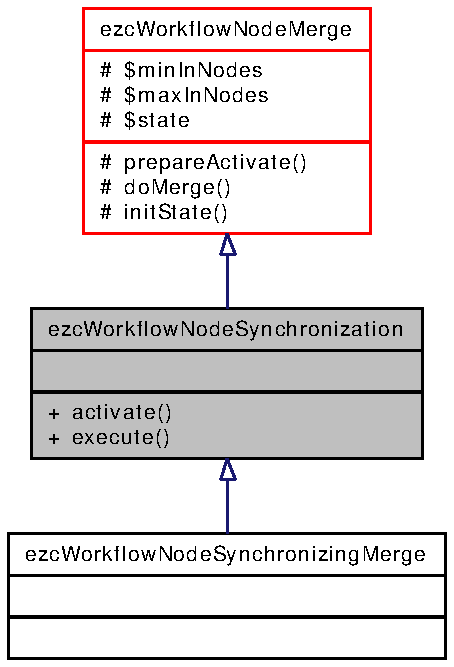
\includegraphics[width=6cm]{figures/WorkflowNodeSynchronization}\\[5mm]
\end{center}
\caption{The \texttt{ezcWorkflowNodeSynchronization} class and its subclasses}
\label{classezcWorkflowNodeSynchronization}
\end{figure}

\subsubsection{ezcWorkflowNodeExclusiveChoice}

\emph{Incoming Nodes: 1}\\
\emph{Outgoing Nodes: 2 \dots *}\\

The \texttt{ezcWorkflowNodeExclusiveChoice} class implements the
\emph{Exclusive Choice} workflow pattern.

\begin{figure}[hbt]
\begin{center}
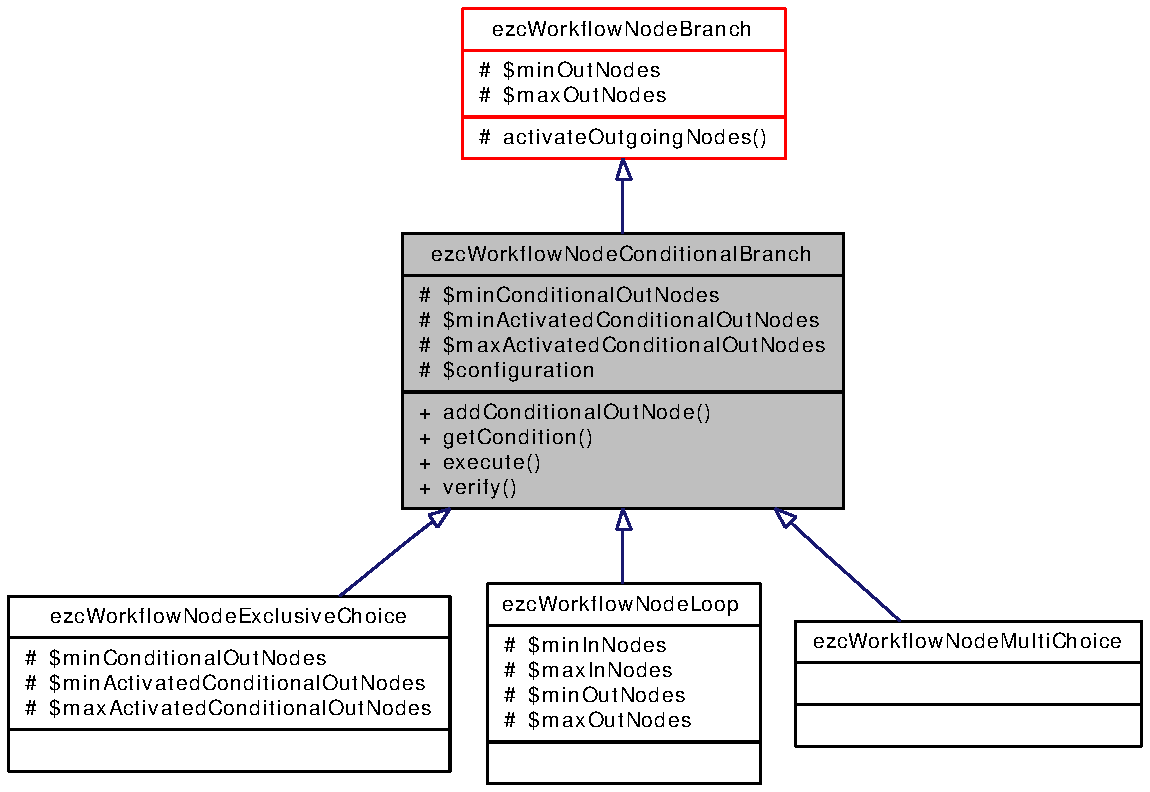
\includegraphics[width=8cm]{figures/WorkflowNodeConditionalBranch}\\[5mm]
\end{center}
\caption{The \texttt{ezcWorkflowNodeConditionalBranch} class and its subclasses}
\label{classezcWorkflowNodeConditionalBranch}
\end{figure}

\subsubsection{ezcWorkflowNodeSimpleMerge}

\emph{Incoming Nodes: 2 \dots *}\\
\emph{Outgoing Nodes: 1}\\

The \texttt{ezcWorkflowNodeSimpleMerge} class implements the \emph{Simple Merge}
workflow pattern.

\subsubsection{ezcWorkflowNodeLoop}

\emph{Incoming Nodes: 2}\\
\emph{Outgoing Nodes: 2}\\

The \texttt{ezcWorkflowNodeLoop} class is a specialization of the
\texttt{ezcWorkflowNodeExclusiveChoice} class and may be used to conveniently
express loops.

\begin{lstlisting}[language=PHP]
$workflow = new ezcWorkflow( 'IncrementingLoop' );

$set  = new ezcWorkflowNodeVariableSet( array( 'i' => 1 ) );
$step = new ezcWorkflowNodeVariableIncrement( 'i' );

$break = new ezcWorkflowConditionVariable(
  'i', new ezcWorkflowConditionIsEqual( 10 )
);

$continue = new ezcWorkflowConditionVariable(
  'i', new ezcWorkflowConditionIsLessThan( 10 )
);

$workflow->startNode->addOutNode( $set );

$loop = new ezcWorkflowNodeLoop;
$loop->addInNode( $set )
       addInNode( $step )
       addConditionalOutNode( $continue, $step )
       addConditionalOutNode( $break, $workflow->endNode );
\end{lstlisting}

The code above is equivalent to a \texttt{for}-loop that iterates the variable
\texttt{i} from \texttt{1} to \texttt{10}.

\subsubsection{ezcWorkflowNodeMultiChoice}

\emph{Incoming Nodes: 1}\\
\emph{Outgoing Nodes: 2 \dots *}\\

The \texttt{ezcWorkflowNodeMultiChoice} class implements the \emph{Multi-Choice}
workflow pattern.

\subsubsection{ezcWorkflowNodeSynchronizingMerge}

\emph{Incoming Nodes: 2 \dots *}\\
\emph{Outgoing Nodes: 1}\\

The \texttt{ezcWorkflowNodeSynchronizingMerge} class implements the
\emph{Synchronizing Merge} workflow pattern.

\subsubsection{ezcWorkflowNodeDiscriminator}

\emph{Incoming Nodes: 2 \dots *}\\
\emph{Outgoing Nodes: 1}\\

The \texttt{ezcWorkflowNodeDiscriminator} class implements the
\emph{Discriminator} workflow pattern.


\section{Condition Classes}
\label{section-ConditionClasses}

The \texttt{ezcWorkflowCondition} classes can be used to express branch
conditions and input validation.

\subsection{Variable Access}

\subsubsection{ezcWorkflowConditionVariable}

An object of the \texttt{ezcWorkflowConditionVariable} class decorates another\\
\texttt{ezcWorkflowCondition} object and applies it condition to a workflow
variable.

\begin{lstlisting}[language=PHP]
$condition = new ezcWorkflowConditionVariable(
  'foo', new ezcWorkflowConditionIsTrue
);
\end{lstlisting}

\subsubsection{ezcWorkflowConditionVariables}

An object of the \texttt{ezcWorkflowConditionVariables} class decorates an\\
\texttt{ezcWorkflowConditionComparison} object and applies it to two workflow
variables.

\begin{lstlisting}[language=PHP]
$condition = new ezcWorkflowConditionVariables(
  'foo', 'bar', new ezcWorkflowConditionIsEqual
);
\end{lstlisting}

\subsection{Boolean Expressions}

\subsubsection{ezcWorkflowConditionNot}

An object of the \texttt{ezcWorkflowConditionNot} class decorates an
\texttt{ezcWorkflowCondition} object and negates its expression.

\begin{lstlisting}[language=PHP]
$notNondition = new ezcWorkflowConditionNot( $condition );
\end{lstlisting}

\subsubsection{ezcWorkflowConditionAnd}

An object of the \texttt{ezcWorkflowConditionAnd} class represents a
boolean \emph{AND} expression. It can hold an arbitrary number of
\texttt{ezcWorkflowCondition} objects.

\begin{lstlisting}[language=PHP]
$and = new ezcWorkflowConditionAnd( array( $condition, ... ) );
\end{lstlisting}

\subsubsection{ezcWorkflowConditionOr}

An object of the \texttt{ezcWorkflowConditionOr} class represents a
boolean \emph{OR} expression. It can hold an arbitrary number of
\texttt{ezcWorkflowCondition} objects.

\begin{lstlisting}[language=PHP]
$or = new ezcWorkflowConditionOr( array( $condition, ... ) );
\end{lstlisting}

\subsubsection{ezcWorkflowConditionXor}

An object of the \texttt{ezcWorkflowConditionXor} class represents a
boolean \emph{XOR} expression. It can hold an arbitrary number of
\texttt{ezcWorkflowCondition} objects.

\begin{lstlisting}[language=PHP]
$xor = new ezcWorkflowConditionXor( array( $condition, ... ) );
\end{lstlisting}

\subsection{Comparisons}

\subsubsection{ezcWorkflowConditionIsTrue}

The condition represented by an \texttt{ezcWorkflowConditionIsTrue} object
evaluates to \texttt{true} when the associated workflow variable has the
value \texttt{true}.

\begin{lstlisting}[language=PHP]
$condition = new ezcWorkflowConditionVariable(
  'variable name',
  new ezcWorkflowConditionIsTrue
);
\end{lstlisting}

\subsubsection{ezcWorkflowConditionIsFalse}

The condition represented by an \texttt{ezcWorkflowConditionIsFalse} object
evaluates to \texttt{true} when the associated workflow variable has the
value \texttt{false}.

\begin{lstlisting}[language=PHP]
$condition = new ezcWorkflowConditionVariable(
  'variable name',
  new ezcWorkflowConditionIsFalse
);
\end{lstlisting}

\subsubsection{ezcWorkflowConditionIsEqual}

The condition represented by an \texttt{ezcWorkflowConditionIsEqual} object
evaluates to \texttt{true} when the associated workflow variable is equal to
the comparison value.

\begin{lstlisting}[language=PHP]
$condition = new ezcWorkflowConditionVariable(
  'variable name',
  new ezcWorkflowConditionIsEqual( $comparisonValue )
);
\end{lstlisting}

\subsubsection{ezcWorkflowConditionIsNotEqual}

The condition represented by an \texttt{ezcWorkflowConditionIsNotEqual} object
evaluates to \texttt{true} when the associated workflow variable is not equal
to the comparison value.

\begin{lstlisting}[language=PHP]
$condition = new ezcWorkflowConditionVariable(
  'variable name',
  new ezcWorkflowConditionIsNotEqual( $comparisonValue )
);
\end{lstlisting}

\subsubsection{ezcWorkflowConditionIsGreaterThan}

The condition represented by an \texttt{ezcWorkflowConditionIsGreaterThan}
object evaluates to \texttt{true} when the associated workflow variable is
greater than the comparison value.

\begin{lstlisting}[language=PHP]
$condition = new ezcWorkflowConditionVariable(
  'variable name',
  new ezcWorkflowConditionIsGreaterThan( $comparisonValue )
);
\end{lstlisting}

\subsubsection{ezcWorkflowConditionIsEqualOrGreaterThan}

The condition represented by an \texttt{ezcWorkflowConditionIsEqualOrGreaterThan}
object evaluates to \texttt{true} when the associated workflow variable is
equal or greater than the comparison value.

\begin{lstlisting}[language=PHP]
$condition = new ezcWorkflowConditionVariable(
  'variable name',
  new ezcWorkflowConditionIsEqualOrGreaterThan( $comparisonValue )
);
\end{lstlisting}

\subsubsection{ezcWorkflowConditionIsLessThan}

The condition represented by an \texttt{ezcWorkflowConditionIsLessThan}
object evaluates to \texttt{true} when the associated workflow variable is
less than the comparison value.

\begin{lstlisting}[language=PHP]
$condition = new ezcWorkflowConditionVariable(
  'variable name',
  new ezcWorkflowConditionIsLessThan( $comparisonValue )
);
\end{lstlisting}

\subsubsection{ezcWorkflowConditionIsEqualOrLessThan}

The condition represented by an \texttt{ezcWorkflowConditionIsEqualOrLessThan}
object evaluates to \texttt{true} when the associated workflow variable is
equal or less than the comparison value.

\begin{lstlisting}[language=PHP]
$condition = new ezcWorkflowConditionVariable(
  'variable name',
  new ezcWorkflowConditionIsEqualOrLessThan( $comparisonValue )
);
\end{lstlisting}

\subsection{Types}

\subsubsection{ezcWorkflowConditionIsAnything}

The condition represented by an \texttt{ezcWorkflowConditionIsAnything} object
always evaluates to \texttt{true}.

\begin{lstlisting}[language=PHP]
$condition = new ezcWorkflowConditionVariable(
  'variable name',
  new ezcWorkflowConditionIsAnything
);
\end{lstlisting}

\subsubsection{ezcWorkflowConditionIsArray}

The condition represented by an \texttt{ezcWorkflowConditionIsArray}
object evaluates to \texttt{true} when the associated workflow variable is
an array.

\begin{lstlisting}[language=PHP]
$condition = new ezcWorkflowConditionVariable(
  'variable name',
  new ezcWorkflowConditionIsArray
);
\end{lstlisting}

\subsubsection{ezcWorkflowConditionIsBool}

The condition represented by an \texttt{ezcWorkflowConditionIsBool}
object evaluates to \texttt{true} when the associated workflow variable is
a boolean.

\begin{lstlisting}[language=PHP]
$condition = new ezcWorkflowConditionVariable(
  'variable name',
  new ezcWorkflowConditionIsBool
);
\end{lstlisting}

\subsubsection{ezcWorkflowConditionIsFloat}

The condition represented by an \texttt{ezcWorkflowConditionIsFloat}
object evaluates to \texttt{true} when the associated workflow variable is
a float.

\begin{lstlisting}[language=PHP]
$condition = new ezcWorkflowConditionVariable(
  'variable name',
  new ezcWorkflowConditionIsFloat
);
\end{lstlisting}

\subsubsection{ezcWorkflowConditionIsInteger}

The condition represented by an \texttt{ezcWorkflowConditionIsInteger}
object evaluates to \texttt{true} when the associated workflow variable is
an integer.

\begin{lstlisting}[language=PHP]
$condition = new ezcWorkflowConditionVariable(
  'variable name',
  new ezcWorkflowConditionIsInteger
);
\end{lstlisting}

\subsubsection{ezcWorkflowConditionIsObject}

The condition represented by an \texttt{ezcWorkflowConditionIsObject}
object evaluates to \texttt{true} when the associated workflow variable is
an object.

\begin{lstlisting}[language=PHP]
$condition = new ezcWorkflowConditionVariable(
  'variable name',
  new ezcWorkflowConditionIsObject
);
\end{lstlisting}

\subsubsection{ezcWorkflowConditionIsString}

The condition represented by an \texttt{ezcWorkflowConditionIsString}
object evaluates to \texttt{true} when the associated workflow variable is
a string

\begin{lstlisting}[language=PHP]
$condition = new ezcWorkflowConditionVariable(
  'variable name',
  new ezcWorkflowConditionIsString
);
\end{lstlisting}
